
\let\negmedspace\undefined
\let\negthickspace\undefined
\documentclass[journal,12pt,twocolumn]{IEEEtran}
\usepackage{cite}
\usepackage{amsmath,amssymb,amsfonts,amsthm}
\usepackage{algorithmic}
\usepackage{graphicx}
\usepackage{textcomp}
\usepackage{xcolor}
\usepackage{txfonts}
\usepackage{listings}
\usepackage{enumitem}
\usepackage{mathtools}
\usepackage{gensymb}
\usepackage[breaklinks=true]{hyperref}
\usepackage{tkz-euclide} % loads  TikZ and tkz-base
\usepackage{listings}


\newtheorem{theorem}{Theorem}[section]
\newtheorem{problem}{Problem}
\newtheorem{proposition}{Proposition}[section]
\newtheorem{lemma}{Lemma}[section]
\newtheorem{corollary}[theorem]{Corollary}
\newtheorem{example}{Example}[section]
\newtheorem{definition}[problem]{Definition}
%\newtheorem{thm}{Theorem}[section] 
%\newtheorem{defn}[thm]{Definition}
%\newtheorem{algorithm}{Algorithm}[section]
%\newtheorem{cor}{Corollary}
\newcommand{\BEQA}{\begin{eqnarray}}
\newcommand{\EEQA}{\end{eqnarray}}
\newcommand{\define}{\stackrel{\triangle}{=}}
\theoremstyle{remark}
\newtheorem{rem}{Remark}

%\bibliographystyle{ieeetr}
\begin{document}
%

\providecommand{\pr}[1]{\ensuremath{\Pr\left(#1\right)}}
\providecommand{\prt}[2]{\ensuremath{p_{#1}^{\left(#2\right)} }}        % own macro for this question
\providecommand{\qfunc}[1]{\ensuremath{Q\left(#1\right)}}
\providecommand{\sbrak}[1]{\ensuremath{{}\left[#1\right]}}
\providecommand{\lsbrak}[1]{\ensuremath{{}\left[#1\right.}}
\providecommand{\rsbrak}[1]{\ensuremath{{}\left.#1\right]}}
\providecommand{\brak}[1]{\ensuremath{\left(#1\right)}}
\providecommand{\lbrak}[1]{\ensuremath{\left(#1\right.}}
\providecommand{\rbrak}[1]{\ensuremath{\left.#1\right)}}
\providecommand{\cbrak}[1]{\ensuremath{\left\{#1\right\}}}
\providecommand{\lcbrak}[1]{\ensuremath{\left\{#1\right.}}
\providecommand{\rcbrak}[1]{\ensuremath{\left.#1\right\}}}
\newcommand{\sgn}{\mathop{\mathrm{sgn}}}
\providecommand{\abs}[1]{\left\vert#1\right\vert}
\providecommand{\res}[1]{\Res\displaylimits_{#1}} 
\providecommand{\norm}[1]{\left\lVert#1\right\rVert}
%\providecommand{\norm}[1]{\lVert#1\rVert}
\providecommand{\mtx}[1]{\mathbf{#1}}
\providecommand{\mean}[1]{E\left[ #1 \right]}
\providecommand{\cond}[2]{#1\middle|#2}
\providecommand{\fourier}{\overset{\mathcal{F}}{ \rightleftharpoons}}
\newenvironment{amatrix}[1]{%
  \left(\begin{array}{@{}*{#1}{c}|c@{}}
}{%
  \end{array}\right)
}
%\providecommand{\hilbert}{\overset{\mathcal{H}}{ \rightleftharpoons}}
%\providecommand{\system}{\overset{\mathcal{H}}{ \longleftrightarrow}}
	%\newcommand{\solution}[2]{\textbf{Solution:}{#1}}
\newcommand{\solution}{\noindent \textbf{Solution: }}
\newcommand{\cosec}{\,\text{cosec}\,}
\providecommand{\dec}[2]{\ensuremath{\overset{#1}{\underset{#2}{\gtrless}}}}
\newcommand{\myvec}[1]{\ensuremath{\begin{pmatrix}#1\end{pmatrix}}}
\newcommand{\mydet}[1]{\ensuremath{\begin{vmatrix}#1\end{vmatrix}}}
\newcommand{\myaugvec}[2]{\ensuremath{\begin{amatrix}{#1}#2\end{amatrix}}}
\providecommand{\rank}{\text{rank}}
\providecommand{\pr}[1]{\ensuremath{\Pr\left(#1\right)}}
\providecommand{\qfunc}[1]{\ensuremath{Q\left(#1\right)}}
	\newcommand*{\permcomb}[4][0mu]{{{}^{#3}\mkern#1#2_{#4}}}
\newcommand*{\perm}[1][-3mu]{\permcomb[#1]{P}}
\newcommand*{\comb}[1][-1mu]{\permcomb[#1]{C}}
\providecommand{\qfunc}[1]{\ensuremath{Q\left(#1\right)}}
\providecommand{\gauss}[2]{\mathcal{N}\ensuremath{\left(#1,#2\right)}}
\providecommand{\diff}[2]{\ensuremath{\frac{d{#1}}{d{#2}}}}
\providecommand{\myceil}[1]{\left \lceil #1 \right \rceil }
\newcommand\figref{Fig.~\ref}
\newcommand\tabref{Table~\ref}
\newcommand{\sinc}{\,\text{sinc}\,}
\newcommand{\rect}{\,\text{rect}\,}
%%
%	%\newcommand{\solution}[2]{\textbf{Solution:}{#1}}
%\newcommand{\solution}{\noindent \textbf{Solution: }}
%\newcommand{\cosec}{\,\text{cosec}\,}
%\numberwithin{equation}{section}
%\numberwithin{equation}{subsection}
%\numberwithin{problem}{section}
%\numberwithin{definition}{section}
%\makeatletter
%\@addtoreset{figure}{problem}
%\makeatother

%\let\StandardTheFigure\thefigure
\let\vec\mathbf

\bibliographystyle{IEEEtran}


\vspace{3cm}

\title{

\textbf{62.2023} 

}
\author{ ROLL NO:EE22BTECH11027\\
         NAME: KATARI SIRI VARSHINI
	}
	
	

\maketitle

\newpage

%\tableofcontents

\bigskip

\renewcommand{\thefigure}{\theenumi}
\renewcommand{\thetable}{\theenumi}
62.Consider a birth-death process on the state space $\{0, 1, 2, 3\}$. The birth rates are
given by $\lambda_0 = 1$, $\lambda_1 = 1$, $\lambda_2 = 2$, and $\lambda_3 = 0$. The death rates are given by
$\mu_0 = 0$, $\mu_1 = 1$, $\mu_2 = 1$, and $\mu_3 = 1$. If $[\pi_0, \pi_1, \pi_2, \pi_3]$ is the unique
stationary distribution, then $\pi_0 + 2\pi_1 + 3\pi_2 + 4\pi_3$ (rounded off to two decimal places) equals
\\ \solution:
Given, a birth-death process on the state space $\{0, 1, 2, 3\}$ with The birth rates $\lambda_0 = 1$, $\lambda_1 = 1$, $\lambda_2 = 2$, $\lambda_3 = 0$ and the death rates $\mu_0 = 0$, $\mu_1 = 1$, $\mu_2 = 1$, and $\mu_3 = 1$ defined over a stationary distribution $[\pi_0, \pi_1, \pi_2, \pi_3]$.
\begin{figure}[h]
    \centering
    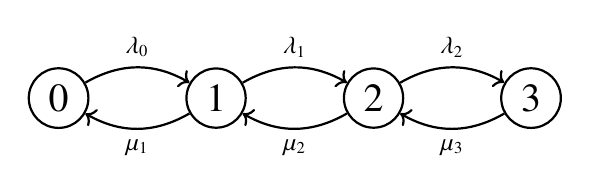
\begin{tikzpicture}[-,auto,node distance=2cm,thick,main node/.style={circle,draw,font=\sffamily\Large\bfseries}]
      \node[main node] (0) {$0$};
      \node[main node] (1) [right of=0] {$1$};
      \node[main node] (2) [right of=1] {$2$};
      \node[main node] (3) [right of=2] {$3$};
  
      \path[every node/.style={font=\sffamily\small}]
        (0) edge [bend left,->] node[above] {$\lambda_0$} (1)
        (1) edge [bend left,->] node[below] {$\mu_1$} (0)
            edge [bend left,->] node[above] {$\lambda_1$} (2)
        (2) edge [bend left,->] node[below] {$\mu_2$} (1)
            edge [bend left,->] node[above] {$\lambda_2$} (3)
        (3) edge [bend left,->] node[below] {$\mu_3$} (2);
    \end{tikzpicture}
    \caption{Markov Chain for Birth-Death Process}
    \label{fig:markov_chain}
\end{figure}
\begin{equation}
\label{eq:62.1}
\text{Let,  }
\pi = \begin{bmatrix}
\pi_0\\
\pi_1\\
\pi_2\\
\pi_3
\end{bmatrix}
\end{equation}
The steady-state balanced solution of the birth and death process is given by
\begin{equation}
\label{eq:62.2}
\begin{split}
\lambda_0\pi_0 &= \mu_1\pi_1 \quad (\text{for } i = 0)\\
(\lambda_i + \mu_i)\pi_i &= \mu_{i+1}\pi_{i+1} + \lambda_{i-1}\pi_{i-1} (i = 1,2,\ldots)
\end{split}
\end{equation}
$\therefore$ Transition Matrix $P$ for the given states is given by 
\begin{equation}
\label{eq:62.3}
\begin{split}
P &= \begin{bmatrix}
-\lambda_0 & \mu_1 & 0 & 0 \\
\lambda_0 & -(\lambda_1 + \mu_1) & \mu_2 & 0 \\
0 & \lambda_1 & -(\lambda_2 + \mu_2) & \mu_3\\
0 & 0 & \lambda_2 & -\mu_3
\end{bmatrix}\\
\implies 
P &= \begin{bmatrix}
-1 & 1 & 0 & 0 \\
1 & -2 & 1 & 0 \\
0 & 1 & -3 & 1\\
0 & 0 & 2 & -1
\end{bmatrix}
\end{split}
\end{equation}
Stationary distribution $\pi$ satisfies,
\begin{equation}
\begin{split}
\label{eq:62.4}
P\pi = 0\\
\Sigma_{i=0}^{3}\pi_i = 1
\end{split}
\end{equation}
Converting $P$ to echelon form we get,
\begin{equation}
\label{eq:62.5}
\begin{bmatrix}
-1 & 1 & 0 & 0 \\
0 & 1 & -1 & 0 \\
0 & 0 & -2 & 1\\
0 & 0 & 0 & 0
\end{bmatrix}
\begin{bmatrix}
\pi_0\\
\pi_1\\
\pi_2\\
\pi_3
\end{bmatrix} =
\begin{bmatrix}
0\\
0\\
0\\
0
\end{bmatrix}
\end{equation}
From the above we get
\begin{equation}
\label{eq:62.6}
\begin{split}
\pi_3 & = 2\pi_2\\
\pi_2 &= \pi_1\\
\pi_1 &= \pi_0\\
\text{from, } \\
\Sigma_{i=0}^{3}\pi_i &= 1\\
\pi_0 &= \frac{1}{5}\\
\therefore
\pi &= \begin{bmatrix}
\frac{1}{5}\\
\frac{1}{5}\\
\frac{1}{5}\\
\frac{2}{5}
\end{bmatrix}
\end{split}
\end{equation}
Using the results obtained in equations from \eqref{eq:62.5}, we get 
\begin{equation}
\therefore \pi_0 + 2\pi_1 + 3\pi_2 + 4\pi_3 = \begin{bmatrix}1\\
2\\
3\\
4
\end{bmatrix}
\cdot \pi = 2.80
\end{equation}
\end{document}

